% =====================================================================
%  Apresentação -- Grupo 8 -- Aprendizagem Profunda -- Módulo 2
%  Classificação de Imagens ERCP com CNNs Profundas
%  Maio de 2026 · Universidade do Minho
% =====================================================================
\documentclass[aspectratio=169]{beamer}

\usepackage[utf8]{inputenc}
\usepackage[T1]{fontenc}
\usepackage{amsmath}
\usepackage{graphicx}
\usepackage{booktabs}
\usepackage{colortbl}
\usepackage{multirow}

% ---- Tema e cores ---------------------------------------------------
\usetheme{Madrid}
\usecolortheme{default}

% Cabeçalho discreto
\setbeamertemplate{navigation symbols}{}
\setbeamertemplate{headline}{}

% Rodapé: grupo | título curto | nº slide
\setbeamertemplate{footline}{%
  \leavevmode\hbox{%
    \begin{beamercolorbox}[wd=.25\paperwidth,ht=2.5ex,dp=1ex,center]{author in head/foot}%
      \usebeamerfont{author in head/foot}Grupo 8 --- UMinho
    \end{beamercolorbox}%
    \begin{beamercolorbox}[wd=.5\paperwidth,ht=2.5ex,dp=1ex,center]{title in head/foot}%
      \usebeamerfont{title in head/foot}Classificação ERCP com CNNs
    \end{beamercolorbox}%
    \begin{beamercolorbox}[wd=.25\paperwidth,ht=2.5ex,dp=1ex,right]{date in head/foot}%
      \usebeamerfont{date in head/foot}
      \insertframenumber{} / \inserttotalframenumber\hspace*{1em}
    \end{beamercolorbox}%
  }%
}

% Cores de destaque
\definecolor{umred}{RGB}{180,20,20}
\setbeamercolor{alerted text}{fg=umred}
\setbeamercolor{block title}{bg=umred!80!black,fg=white}

% ---- Metadados ------------------------------------------------------
\title[Classificação ERCP com CNNs]{%
  Classificação de Imagens ERCP\\
  com Redes Neurais Convolucionais Profundas}
\subtitle{Comparativo: DenseNet121 \textbullet{} ResNet50 \textbullet{}
          MobileNetV2 \textbullet{} EfficientNet-B7}
\author[Grupo 8: Bergueira, Silva, Pereira, Rodrigues]{%
  C.\ Bergueira (pg11605@alunos.uminho.pt) \and D.\ Silva (pg59999@alunos.uminho.pt) \and\\ F.\ Pereira (pg42201@alunos.uminho.pt) \and R.\ Rodrigues (pg7942@alunos.uminho.pt)}
\institute[UMinho]{%
  Universidade do Minho --- Grupo 8\\[4pt]
  \small Aprendizagem Profunda - Módulo 2 - 2025/2026}
\date{2026}

% =====================================================================
\begin{document}
% =====================================================================

% ------ SLIDE 1: Título ----------------------------------------------
\begin{frame}
  \titlepage
\end{frame}

% ------ SLIDE 2: Problema e Dataset ----------------------------------
\begin{frame}{Problema: Classificação Automática de ERCP}
  \begin{columns}[T]
    \column{0.54\textwidth}
      \textbf{Contexto clínico}
      \begin{itemize}
        \item ERCP: fluoroscopia para diagnóstico biliar/pancreático
        \item Interpretação manual é demorada e especializada
        \item Objetivo: sistema CADx de apoio à decisão
      \end{itemize}
      \medskip
      \textbf{Dataset MIQR-CC~(Martins et al., 2025)}
      {\small
      \begin{tabular}{lccc}
        \toprule
        Classe & Treino & Val & Teste \\
        \midrule
        \alert{Biliary Leaks} & 110 (10\%) & 24 & 17 \\
        Lithiasis          & 505 (47\%) & 98 & 123 \\
        Normal             & 197 (18\%) & 59 & 43 \\
        Stricture          & 255 (24\%) & 53 & 84 \\
        \midrule
        \textbf{Total}     & \textbf{1067} & 234 & 267 \\
        \bottomrule
      \end{tabular}
      }
    \column{0.46\textwidth}
      \begin{alertblock}{Desafio central: desequilíbrio}
        47\% Lithiasis \textbf{vs.} 10\% Biliary Leaks\\[4pt]
        Um modelo que ignore BL alcança accuracy alta
        mas é \textbf{fortemente penalizado} pela métrica.
      \end{alertblock}
      \medskip
      \textbf{Métrica: F1-Score Macro}
      \[
        F_1^{\text{macro}} = \frac{1}{4}\sum_{c=1}^{4}
        \frac{2\,P_c R_c}{P_c + R_c}
      \]
      \small Peso igual por classe --- independente da frequência.
  \end{columns}
\end{frame}

% ------ SLIDE 3: Arquiteturas ----------------------------------------
\begin{frame}{4 Arquiteturas CNN -- Transfer Learning a partir do ImageNet}
  \begin{columns}[T]
    \column{0.245\textwidth}
      \begin{block}{DenseNet121}
        $\mathbf{x}_L = H_L([\mathbf{x}_0,\ldots,\mathbf{x}_{L-1}])$\\[4pt]
        \textbf{Conectividade densa}\\
        Reutiliza features de baixo nível em camadas profundas.\\[4pt]
        7M parâmetros
      \end{block}
    \column{0.245\textwidth}
      \begin{block}{ResNet50}
        $\mathbf{x}_{L+1} = \mathcal{F}(\mathbf{x}_L)+\mathbf{x}_L$\\[4pt]
        \textbf{Conexões residuais}\\
        Treino estável; arquitectura de referência desde 2015.\\[4pt]
        25M parâmetros
      \end{block}
    \column{0.245\textwidth}
      \begin{block}{MobileNetV2}
        Depthwise separable\\
        \textbf{Inverted residual}\\
        Leve e eficiente; menor capacidade representacional.\\[4pt]
        3.4M parâmetros
      \end{block}
    \column{0.245\textwidth}
      \begin{block}{EfficientNet-B7}
        $d=\alpha^\phi,\; w=\beta^\phi,\; r=\gamma^\phi$\\[4pt]
        \textbf{Compound scaling}\\
        Maior capacidade mas sobreajuste crítico com $\sim$1000 imagens.\\[4pt]
        66M parâmetros
      \end{block}
  \end{columns}
  \vspace{0.6em}
  \begin{alertblock}{Motivação comum: Transfer Learning}
    Com apenas 1067 imagens de treino, fine-tuning de pesos ImageNet é essencial.
    Treino de raiz seria instável e propenso a overfitting.
  \end{alertblock}
\end{frame}

% ------ SLIDE 4: Técnicas Anti-Desequilíbrio -------------------------
\begin{frame}{Estratégia Metodológica: Tratar o Desequilíbrio}
  \begin{columns}[T]
    \column{0.48\textwidth}
      \textbf{Funções de perda ponderadas}
      \begin{itemize}
        \item \textbf{Focal Loss:}
          $FL(p_t)=-\alpha_t(1-p_t)^\gamma\log p_t$\\
          Penaliza exemplos fáceis; foca nas classes raras.
        \item \textbf{CE ponderada:}
          $w_c = N/(C\cdot N_c)$\\
          Amplifica gradiente de Biliary Leaks.
        \item \textbf{Label smoothing} ($\epsilon=0.1$):
          evita sobreconfiança.
      \end{itemize}
      \medskip
      \textbf{Augmentação e inferência}
      \begin{itemize}
        \item \textbf{Mixup} ($\alpha=0.4$): interpola imagens e labels
        \item \textbf{TTA} (4--8 passes): média de probabilidades
        \item \textbf{Threshold tuning} por classe (val set)
      \end{itemize}
    \column{0.52\textwidth}
      \textbf{Pré-processamento}
      \begin{itemize}
        \item \textbf{CLAHE offline} (clipLimit=2, 8$\times$8):\\
          equalização adaptativa --- realça estruturas subtis
        \item Normalização ImageNet
          ($\mu=[0.485, 0.456, 0.406]$)
      \end{itemize}
      \medskip
      \textbf{Optimizadores}
      \begin{itemize}
        \item AdamW + OneCycleLR (DenseNet)
        \item Differential LRs backbone/head (MobileNet)
        \item BN frozen nos últimos blocos (EfficientNet)
      \end{itemize}
      \medskip
      \begin{alertblock}{Impacto real (DenseNet, caso de estudo)}
        \begin{tabular}{lc}
          Estratégia anti-desequilíbrio & \alert{+10.2 pp}\\
          CLAHE offline + AMP + 256 px  & \alert{+6.1 pp}\\
        \end{tabular}
      \end{alertblock}
  \end{columns}
\end{frame}

% ------ SLIDE 5: Resultados Globais ----------------------------------
\begin{frame}{Resultados no Conjunto de Teste (n=267)}
  \begin{center}
    \begin{tabular}{lcccc}
      \toprule
      Modelo & F1 Macro & Accuracy & AUC-ROC & F1 BL\\
      \midrule
      \rowcolor{umred!15}
      \alert{\textbf{DenseNet121 v100}} &
        \alert{\textbf{0.7076}} & \alert{\textbf{0.7266}} &
        $\sim$0.92 & \alert{\textbf{0.667}}\\
      ResNet50 v2    & 0.6647 & 0.7041 & $\sim$0.89 & 0.552\\
      EfficientNet-B7 RR12 & 0.555 & 0.633  & $\sim$0.87 & 0.286\\
      MobileNetV2 v4 & $\sim$0.556 & $\sim$0.620 & $\sim$0.86 & 0.261\\
      \midrule
      \textit{Baseline artigo (MIQR-CC)} &
        \textit{0.738} & \textit{---} & \textit{---} & \textit{---}\\
      \bottomrule
    \end{tabular}
  \end{center}
  \vspace{0.4em}
  \begin{columns}
    \column{0.5\textwidth}
      \begin{block}{Ganho interno: v0 $\to$ v100}
        $0.545 \xrightarrow{+10.2\,\text{pp}} 0.647
         \xrightarrow{+6.1\,\text{pp}} \mathbf{0.7076}$
      \end{block}
    \column{0.5\textwidth}
      \begin{alertblock}{vs.\ Baseline publicada}
        DenseNet v100 fica \textbf{--3.0 pp} abaixo de 0.738\\
        (Martins et al., MIQR-CC 2025).
      \end{alertblock}
  \end{columns}
\end{frame}

% ------ SLIDE 6: F1 por Classe ---------------------------------------
\begin{frame}{F1, Precisão e Recall por Classe}
  \begin{center}
    \resizebox{\textwidth}{!}{%
    \begin{tabular}{l|ccc|ccc|ccc|ccc}
      \toprule
      & \multicolumn{3}{c|}{DenseNet121}
      & \multicolumn{3}{c|}{ResNet50}
      & \multicolumn{3}{c|}{EfficientNet}
      & \multicolumn{3}{c}{MobileNet} \\
      Classe & P & R & F1 & P & R & F1 & P & R & F1 & P & R & F1 \\
      \midrule
      \alert{Biliary Leaks}
        & 0.900 & 0.529 & \textbf{0.667}
        & 0.667 & 0.471 & 0.552
        & 0.364 & 0.235 & 0.286
        & 0.500 & 0.176 & 0.261\\
      Lithiasis
        & 0.783 & 0.675 & 0.725
        & 0.824 & 0.683 & \textbf{0.747}
        & 0.631 & 0.724 & 0.674
        & 0.664 & 0.772 & 0.714\\
      Normal
        & 0.615 & 0.744 & 0.674
        & 0.443 & 0.907 & 0.595
        & 0.577 & 0.698 & 0.633
        & 0.545 & 0.558 & 0.552 \\
      Stricture
        & 0.707 & 0.833 & \textbf{0.765}
        & 0.877 & 0.679 & \textbf{0.765}
        & 0.730 & 0.548 & 0.626
        & 0.743 & 0.655 & 0.696 \\
      \midrule
      \textbf{Macro}
        & & & \textbf{0.708}
        & & & 0.665
        & & & 0.555
        & & & 0.556\\
      \bottomrule
    \end{tabular}%
    }
  \end{center}
  \vspace{0.3em}
  \begin{columns}
    \column{0.5\textwidth}
      \alert{Biliary Leaks}: recall máximo 9/17 (DenseNet).\\
      Falso negativo = fuga biliar não detectada.
    \column{0.5\textwidth}
      \alert{Stricture $\to$ Lithiasis}: confusão sistemática.\\
      Tratamento erróneo se mal classificado.
  \end{columns}
\end{frame}

% ------ SLIDE 7: Matrizes de Confusão --------------------------------
\begin{frame}{Matrizes de Confusão: Dois Melhores Modelos}
  \begin{columns}[T]
    \column{0.48\textwidth}
      \begin{center}
      \textbf{DenseNet121 v100} \quad F1 = 0.7076\\[4pt]
      {\small
      \begin{tabular}{lccccc}
        \toprule
        & & \multicolumn{4}{c}{\textit{Predição}}\\
        & & BL & Li & No & St\\
        \midrule
        \multirow{4}{*}{\rotatebox{90}{\textit{Real}}}
        & BL [17] & \textbf{9}  &  1 &  3 &  4\\
        & Li[123] &  1 & \textbf{83} & 17 & 22\\
        & No [43] &  0 &  8 & \textbf{32} &  3\\
        & St [84] &  0 & \alert{14} &  0 & \textbf{70}\\
        \bottomrule
      \end{tabular}
      }
      \end{center}
    \column{0.04\textwidth}
    \column{0.48\textwidth}
      \begin{center}
      \textbf{ResNet50 v2} \quad F1 = 0.6647\\[4pt]
      {\small
      \begin{tabular}{lccccc}
        \toprule
        & & \multicolumn{4}{c}{\textit{Predição}}\\
        & & BL & Li & No & St\\
        \midrule
        \multirow{4}{*}{\rotatebox{90}{\textit{Real}}}
        & BL [17] & \textbf{8}  &  1 &  8 &  0\\
        & Li[123] &  4 & \textbf{84} & 29 &  6\\
        & No [43] &  0 &  2 & \textbf{39} &  2\\
        & St [84] &  0 & \alert{15} & 12 & \textbf{57}\\
        \bottomrule
      \end{tabular}
      }
      \end{center}
  \end{columns}
  \vspace{0.5em}
  \small
  \textbf{Padrão crítico em ambos:} Stricture $\to$ Lithiasis
  (DenseNet: 14/84; ResNet: 15/84). Estrutura tubular da estenose visualmente
  semelhante a depósitos de cálculos em fluoroscopia.\\
  \textbf{DenseNet:} melhor recall de Biliary Leaks (9 vs 8) e recall de
  Stricture (70/84 = 83\%).
\end{frame}

% ------ SLIDE 8: Grad-CAM -------------------------------------------
\begin{frame}{Grad-CAM: Interpretabilidade das Decisões}
  \begin{columns}[T]
    \column{0.5\textwidth}
      \centering
      {\small\textcolor{green!50!black}{\textbf{Correcto}} ---
       Biliary Leaks (52.4\%)}\\[3pt]
      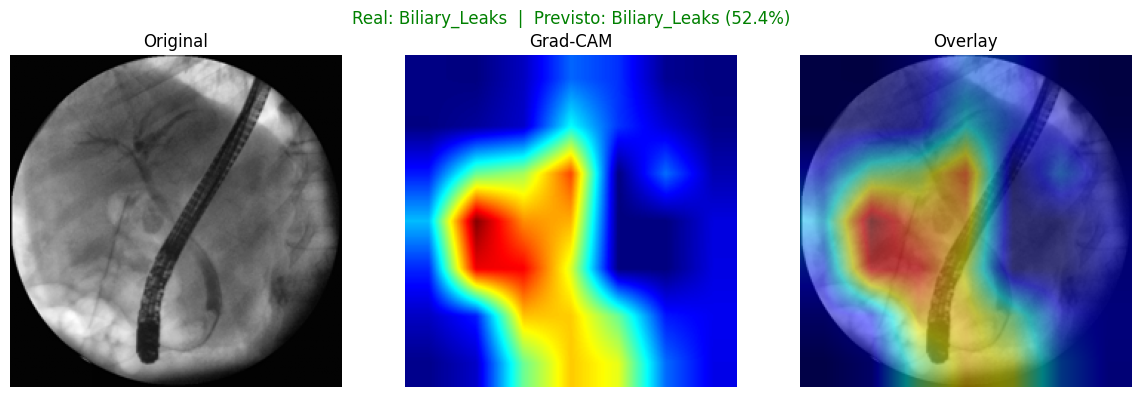
\includegraphics[width=\textwidth]{images/biliaryleaks-correct-grad-cam.png}
      \vspace{4pt}
      {\small\textcolor{green!50!black}{\textbf{Correcto}} ---
       Lithiasis (84.8\%)}\\[3pt]
      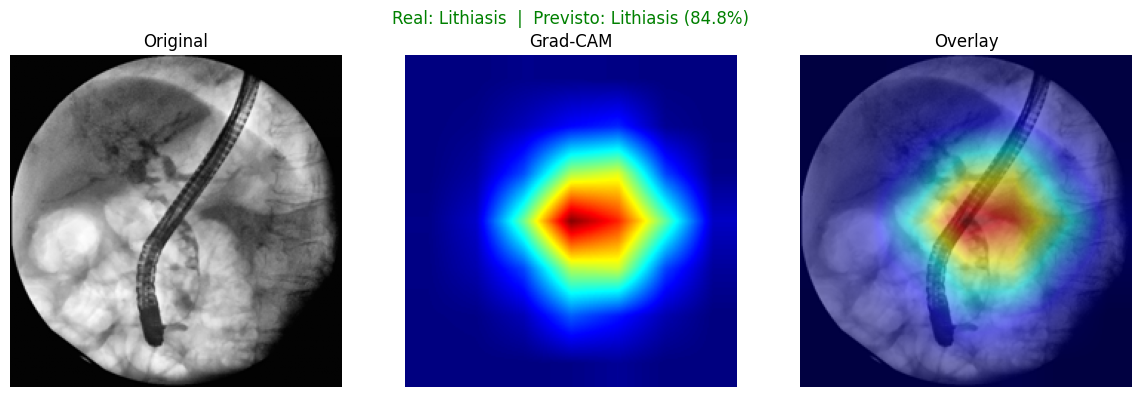
\includegraphics[width=\textwidth]{images/lithiasis-correct-grad-cam.png}
    \column{0.5\textwidth}
      \centering
      {\small\textcolor{red!70!black}{\textbf{Incorrecto}} ---
       Stricture $\to$ Lithiasis (37.4\%)}\\[3pt]
      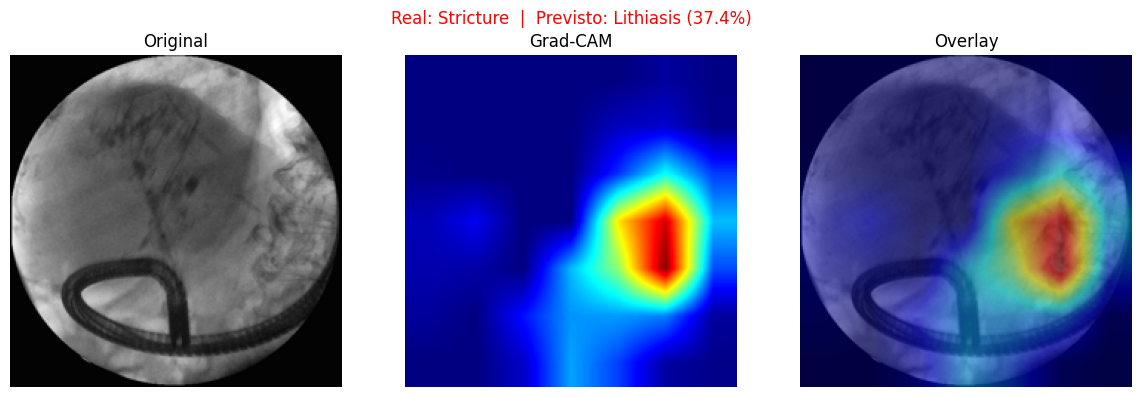
\includegraphics[width=\textwidth]{images/stricture-wrong-grad-cam.png}
      \vspace{4pt}
      {\small\textcolor{red!70!black}{\textbf{Incorrecto}} ---
       Biliary Leaks $\to$ Lithiasis (47.3\%)}\\[3pt]
      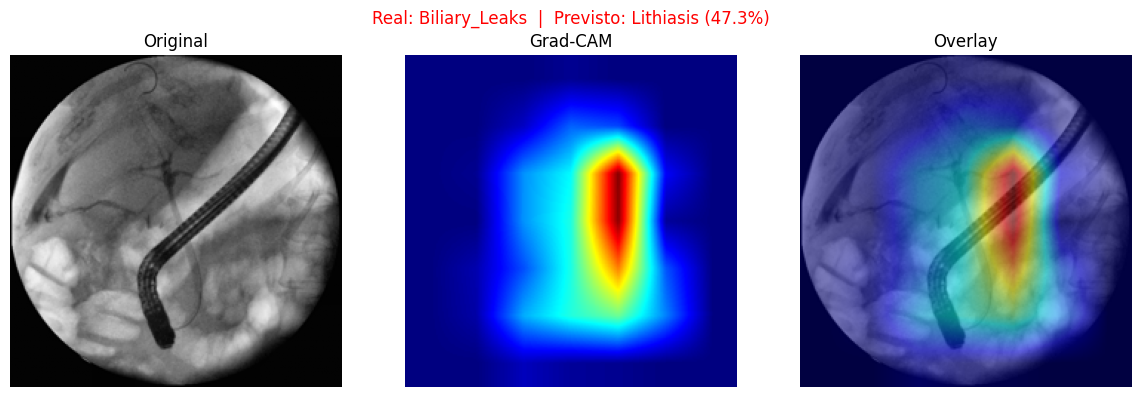
\includegraphics[width=\textwidth]{images/biliaryleaks-wrong-grad-cam.png}
  \end{columns}
\end{frame}

% ------ SLIDE 9: Ensemble --------------------------------------------
\begin{frame}{Ensemble por Soft Voting}
  \begin{columns}[T]
    \column{0.48\textwidth}
      \textbf{Combinação DenseNet + EfficientNet}
      \[
        P_{\text{ens}}(c\mid x)
        = \frac{1}{2}\bigl[P_{\text{Dense}}(c\mid x)
                         + P_{\text{Eff}}(c\mid x)\bigr]
      \]
      \begin{itemize}
        \item As duas arquitecturas cometem erros em padrões distintos
        \item A média suaviza predições incertas
        \item Resultado preliminar (modelos base):\\
          F1 $>$ 0.55 vs.\ 0.545 / 0.480 isolados
      \end{itemize}
      \medskip
      \begin{block}{Próximo passo}
        \small
        Ensemble \textbf{DenseNet v100 + ResNet v2}\\
        (seria o candidato mais forte)
      \end{block}
    \column{0.52\textwidth}
      \textbf{Por que os modelos são complementares?}
      \begin{itemize}
        \item DenseNet: melhor recall BL (9/17) e Stricture (70/84)
        \item ResNet: melhor recall Normal (39/43) e precisão Lithiasis (0.824)
        \item EfficientNet: maior recall Lithiasis (0.724)
      \end{itemize}
      \medskip
      \textbf{Estratégia de pesagem proposta}\\
      \begin{tabular}{lc}
        \toprule
        Modelo & Peso \\
        \midrule
        DenseNet121 v100 & 0.50 \\
        ResNet50 v2 & 0.50 \\
        \bottomrule
      \end{tabular}\\[4pt]
      \small Pode ser optimizado no val set por classe.
  \end{columns}
\end{frame}

% ------ SLIDE 10: Conclusões -----------------------------------------
\begin{frame}{Conclusões e Trabalho Futuro}
  \begin{columns}[T]
    \column{0.52\textwidth}
      \textbf{Ranking Final}\\[4pt]
      {\small
      \begin{tabular}{clcc}
        \toprule
        Pos. & Modelo & F1 & Acc\\
        \midrule
        \alert{1} & \alert{DenseNet121 v100} & \alert{\textbf{0.708}} & \alert{\textbf{0.727}}\\
        2 & ResNet50 v2        & 0.665 & 0.704\\
        3 & EfficientNet-B7    & 0.555 & 0.633\\
        4 & MobileNetV2        & 0.556 & 0.620\\
        \midrule
        -- & \textit{Baseline} & \textit{0.738} & \textit{---}\\
        \bottomrule
      \end{tabular}
      }
      \vspace{0.5em}

      \begin{alertblock}{Conclusão principal}
        \textbf{Tratar o desequilíbrio} (Focal Loss + Mixup + TTA)
        foi $\mathbf{\approx 25\times}$ mais impactante do que
        ajustar resolução ou contraste isoladamente.
      \end{alertblock}
    \column{0.48\textwidth}
      \textbf{Trabalho Futuro}
      \begin{itemize}
        \item \textbf{Ensemble} DenseNet v100 + ResNet v2
        \item \textbf{Síntese de dados} (GAN) para Biliary Leaks\\
          (recall persistente em 9/17)
        \item \textbf{WeightedRandomSampler} dedicado a BL
        \item \textbf{Vision Transformers} (ViT/Swin)
        \item \textbf{Validação cruzada} estratificada k-fold
      \end{itemize}
      \medskip
      \begin{block}{Gap vs.\ Baseline}
        --3.0 pp face a Martins et al.\ (0.738).\\
        Superar requer dados adicionais ou\\
        arquitecturas de atenção espacial.
      \end{block}
  \end{columns}
\end{frame}

% ------ SLIDE 11: Fim ------------------------------------------------
\begin{frame}[plain]
  \begin{center}
    \vspace{1.5em}
    {\LARGE\textbf{Obrigado pela atenção!}}\\[1.2em]
    \large Questões?\\[2em]
    \begin{tabular}{ll}
      \textbf{Melhor modelo:}  & DenseNet121 v100 --- F1 macro = 0.7076 \\[4pt]
      \textbf{Baseline artigo:} & F1 = 0.738 (Martins et al., 2025) \\[4pt]
      \textbf{Ganho interno:}  & $+16.3$ pp (v0 $\to$ v100) \\[4pt]
      \textbf{Semente aleatória:} & 42 (reprodutível) \\[4pt]
      \textbf{Código:} & Repositório GitHub do grupo \\
    \end{tabular}
  \end{center}
\end{frame}

\end{document}
